


\documentclass[a4paper,12pt,spanish]{article}

\usepackage[utf8]{inputenc}


\usepackage{blindtext}
%\usepackage{microtype}
\usepackage{amsfonts, amsmath, amsthm, amssymb}
%\usepackage{fancyhdr}
%\usepackage{index}
%\usepackage{multicol}    

%\usepackage{booktabs}

\usepackage[T1]{fontenc}
\usepackage[utf8]{inputenc}
\usepackage{graphicx}
\usepackage[spanish,es-tabla]{babel}
\usepackage{url}
\usepackage{enumitem}

\usepackage[unicode=true, pdfusetitle,
bookmarks=true,bookmarksnumbered=false,bookmarksopen=false,
breaklinks=true,pdfborder={0 0 1},backref=false,colorlinks=false]
{hyperref}

\usepackage{listings}
\usepackage{longtable}


\usepackage{siunitx} %para el sistema internacional
\usepackage[export]{adjustbox}
\usepackage{booktabs} 
\usepackage{subcaption}

\usepackage{float}


\newcommand{\address}[1]{
	\par {\raggedright #1
		\vspace{1.4em}
		\noindent\par}
}

\usepackage[table,xcdraw]{xcolor}


\pagenumbering{gobble}
\include{noNumberPage}
\pagenumbering{arabic}
\setcounter{page}{1}

%tutorial de tablas latex: https://manualdelatex.com/tutoriales/tablas

\usepackage{multirow}

% \usepackage[table,xcdraw]{xcolor}


%Inicio del documento (hasta que se cierre con \end{document}
\begin{document}
	
	
	% El PDF de salida debe llamarse "memoria_resultados.pdf".
	\title{PEC Física Computacional}
	
	\author{Adrián Rivero Fernández}
	\date{\today}
	
	\maketitle
	
	%\vspace{\baselineskip}
	
	\section{Introducción y objetivos}

	Consistirá en una breve
descripción de lo que se pretende calcular o simular , introduciendo (si fuera necesario) los
conceptos teóricos y las expresiones matemáticas que se van a utilizar. No debe ser una
copia del enunciado.



	\section{Desarrollo y resultados.}
	
	\subsection{Ejercicio 1}
	
	
	
	\begin{figure}[H]
		\centering
		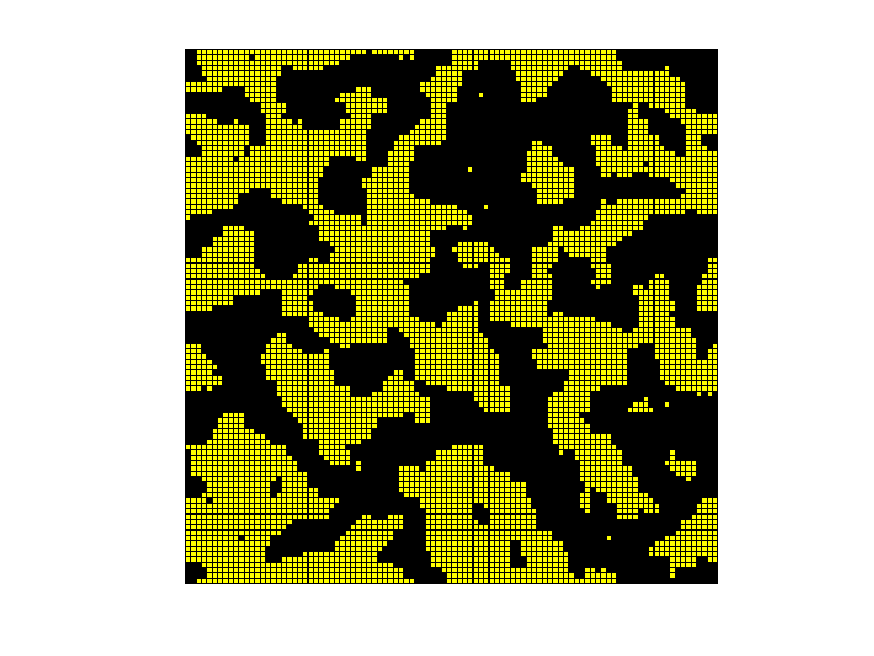
\includegraphics[width=0.7\linewidth]{../obtencion_resultados/a}
		\caption{Disposición para T=1 y 10$^5$ volteos}
		\label{fig:a}
	\end{figure}


	\begin{figure}[H]
		\centering
		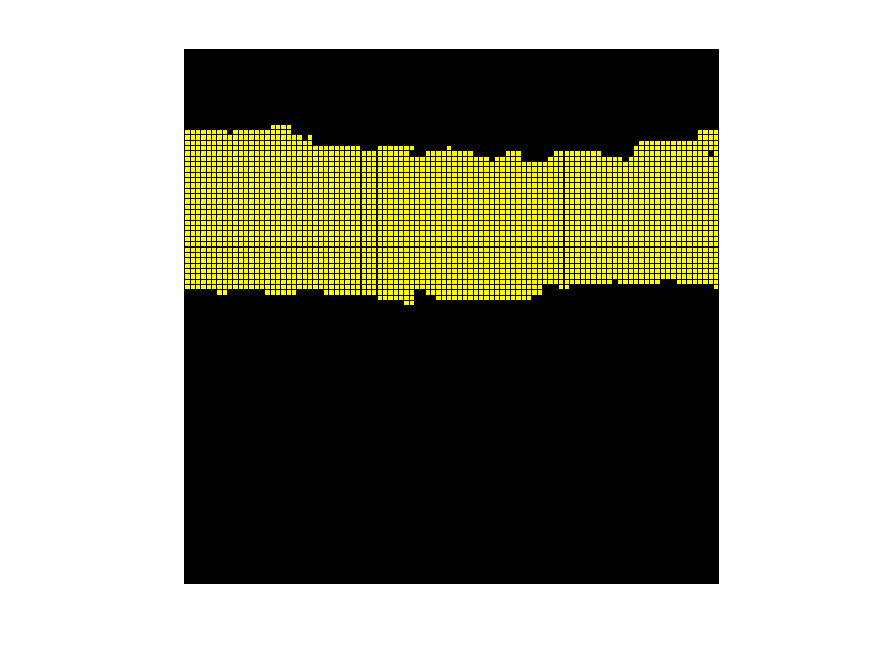
\includegraphics[width=0.7\linewidth]{../obtencion_resultados/b}
		\caption{Disposición para T=1 y 10$^8$ volteos}
		\label{fig:b}
	\end{figure}


	\begin{figure}[H]
		\centering
		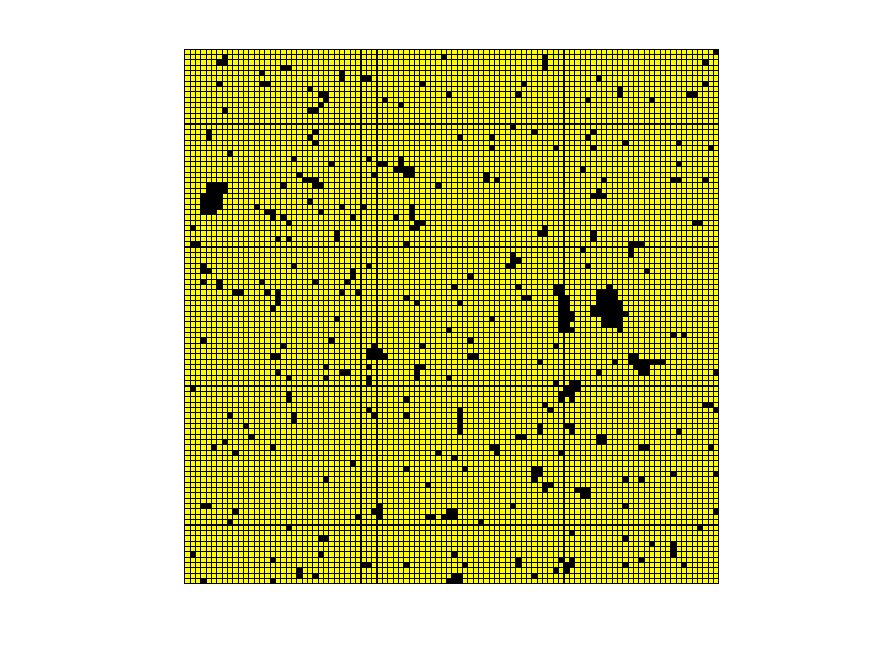
\includegraphics[width=0.7\linewidth]{../obtencion_resultados/c}
		\caption{Disposición para T=2 y 10$^8$ volteos}
		\label{fig:c}
	\end{figure}


	\begin{figure}[H]
		\centering
		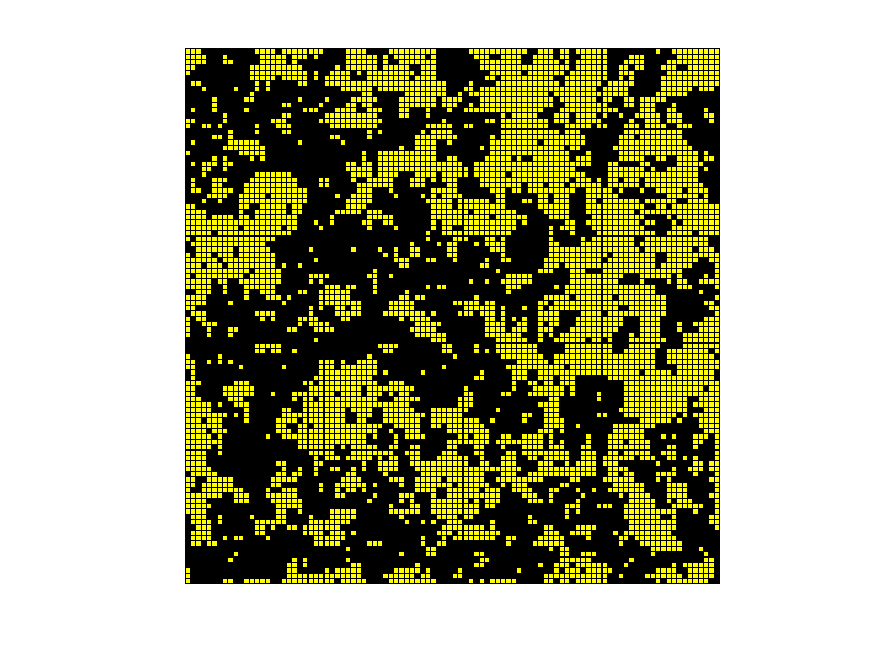
\includegraphics[width=0.7\linewidth]{../obtencion_resultados/d}
		\caption{Disposición para T=2.5 y 10$^8$ volteos}
		\label{fig:d}
	\end{figure}
	
	
	
	
	\subsection{Ejercicio 2}
	
	
	
	\begin{figure}[H]
		\centering
		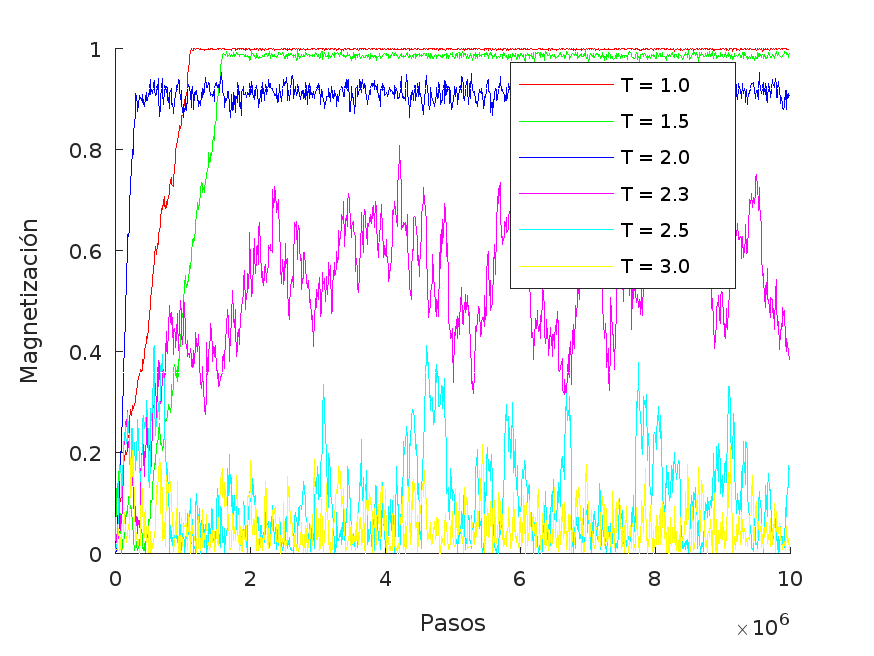
\includegraphics[width=0.7\linewidth]{../obtencion_resultados/grafica_ej2}
		\caption{Magnetización según la cantidad de pasos para distintas temperaturas}
		\label{fig:graficaej2}
	\end{figure}
	
	
	
	
	\subsection{Ejercicio 3}
	
	
	\begin{figure}[H]
		\centering
		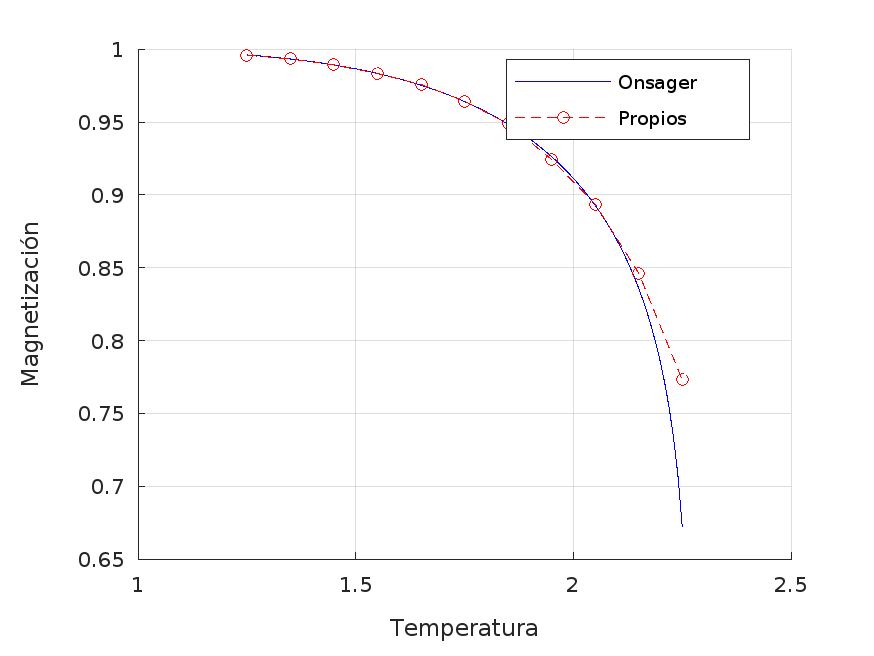
\includegraphics[width=0.7\linewidth]{../obtencion_resultados/grafica_ej3}
		\caption{Evolución de la magnetización media con la temperatura}
		\label{fig:graficaej3}
	\end{figure}
	
	
	
	

	En esta parte se deben mostrar
los resultados obtenidos, y explicar brevemente cómo se han obtenido. Si no se pide
explícitamente en el enunciado del ejercicio


	\section{Análisis y conclusiones.}

	Se deben analizar y explicar los resultados obtenidos en relación a
la teoría presentada en el enunciado de la PEC y los objetivos marcados en el enunciado
del ejercicio. Si los resultados resultan ser incorrectos, el apartado anterior puede estar mal,
pero si se da una posible explicación de ese fallo, este apartado puede estar bien y
compensar la calificación.

	
	
	
	
	
\end{document}




